\documentclass[12pt, letterpaper]{article}
\usepackage[table]{xcolor}
\usepackage{graphicx} % Required for inserting images
\usepackage{titlesec}
\usepackage{float}
\usepackage{amsmath}
\usepackage{layout}
\usepackage{anyfontsize}
\usepackage{listings}
\usepackage{xcolor}
\usepackage{booktabs}
\usepackage{pdflscape}
\usepackage{lscape}
\usepackage{tabularx}
\usepackage{boldline}
\usepackage{tabulary}
\usepackage{tcolorbox}
\usepackage{hyperref}
\usepackage[spanish]{babel}
\usepackage{amssymb} % Añadido para simbolos extra

\usepackage[left=3.5cm, right=3.5cm, top=2.5cm, bottom=2.5cm]{geometry}

\begin{document}

\begin{titlepage}
    \centering
    {\Huge \textsc{\textbf{}}\par}
    \par\vspace{1cm}
    % Asegúrate de tener el archivo de imagen o comenta la línea si no lo tienes
    \begin{figure}[H]
    \begin{minipage}{0.15\textwidth}
        \centering
        
\includegraphics[width=\textwidth]{Logo_UPC.svg.png}
    \end{minipage}
    \hspace{0.02\textwidth}
    \begin{minipage}{0.85\textwidth}
        \centering
        
\includegraphics[width=\textwidth]{logo-fiblletres-upc-color.png}
    \end{minipage}
    \end{figure}
    
    
    {\Huge \textsc{\textbf{}}\par}
    \vspace{2cm}
    {\huge \textsc{Sistema Inteligente Para la Asistencia en el Desarrollo Estructurado de Código Mediante Spec-Driven Development}\par}
    \vspace{2cm}
    {\Large \textsc{\textbf{Gestió De Projectes - Entregable 1}}\par}
    {\large \textsc{Contexto y Alcance del Proyecto}\par}
    
    \vspace{2cm}
    {\normalsize \textbf{Autor:} {Adrià Cebrián Ruiz}\\ \par}
    {\normalsize \textbf{Director:} {Luis Jonás Cuervo Derqui}\\ \par}
    {\normalsize \textbf{Ponente:} {David Garcia Soriano}\\ \par} 
    {\normalsize \textbf{Tutor GEP:} {Joan Sarda Ferrer}\\ \par}
    
    \vspace{0.5cm}
    {Facultat Informàtica de Barcelona (FIB)}\\
    {\normalsize Menció de Computació - Grau en Enginyeria Informàtica\\ \par}
    25 de febrero de 2026

    \vfill
\end{titlepage}

\tableofcontents
\newpage

\section{Contexto}

\subsection{Introducción}
Estamos viviendo el auge de la \textit{Inteligencia Artificial Generativa}, una época en la que una gran parte de los desarrolladores de software y sus respectivas empresas han incorporado la inteligencia artificial en el día a día para el desarrollo de software. Esto conlleva varios problemas como la falta de interés que tienen algunos desarrolladores para aprender nuevos conocimientos, delegando el razonamiento crítico al modelo, lo que genera el conocido como \textit{slop code}: código funcional pero deficiente en estructura y sostenibilidad.

\subsection{Definición del Problema}

El problema central que este TFG busca resolver es la ausencia de un flujo de trabajo estructurado que discipline y oriente el uso de la IA generativa en el desarrollo de software profesional.

Actualmente, los asistentes de código más populares (GitHub Copilot, Cursor, etc.) operan bajo un paradigma \textit{Code-Driven}: el desarrollador describe vagamente lo que quiere y el modelo genera código de forma inmediata, sin exigir ninguna especificación previa. Este enfoque tiene dos consecuencias directas y documentadas:

\begin{itemize}
    \item \textbf{Generación de \textit{slop code}:} El código producido resuelve el problema inmediato, pero carece de estructura coherente, no sigue los estándares del proyecto y acumula deuda técnica. Al no haber una especificación de referencia, el modelo no puede saber qué es correcto más allá de lo que el usuario describe en ese momento. El resultado es un código difícil de mantener, escalar o auditar.

    \item \textbf{Falta de trazabilidad entre requisitos y código:} Sin un documento de especificación que actúe como fuente de verdad, resulta imposible saber si el código generado cumple realmente con los requisitos del negocio, si ha habido desviaciones respecto al diseño original, o quién tomó qué decisión y cuándo.

    \item \textbf{Barrera de incorporación para nuevos desarrolladores:} La ausencia de documentación estructurada convierte la incorporación de un nuevo miembro al equipo en un proceso lento y costoso. Sin especificaciones claras que expliquen el \textit{porqué} de cada decisión de diseño, el nuevo desarrollador debe deducir la arquitectura y las reglas del proyecto leyendo directamente el código, lo que ralentiza su productividad y aumenta el riesgo de que introduzca cambios inconsistentes con la visión original del sistema.
\end{itemize}

Por otro lado, las herramientas que sí exigen especificación previa (como Spec Kit o AgentOS) presentan el problema opuesto: generan una fricción operativa excesiva, produciendo documentación desproporcionada incluso para cambios pequeños, lo que las hace incompatibles con metodologías ágiles reales.

\textbf{En definitiva, el problema es la inexistencia de una solución de asistencia al desarrollo que equilibre la agilidad de las herramientas \textit{Code-Driven} con la rigurosidad estructural que exige el desarrollo de software profesional y sostenible.} Este TFG propone construir exactamente esa solución.

\subsection{Marco de la empresa}

La empresa \textit{Colb.Ai} es una consultoría que implementa soluciones de IA para sus clientes; además, la empresa misma intenta maximizar el provecho que obtiene de estas herramientas en el desarrollo de sus soluciones de software.

El objetivo de este TFG es implementar un sistema que utilice distintos \textit{frameworks} y modelos de inteligencia artificial para que ayude a los desarrolladores a llevar a cabo la toma de requerimientos, planificación del proyecto, y la organización/documentación del código, con tal de ayudar a la empresa a investigar como comenzar nuevos proyectos, y planificar el proceso de desarrollo. 

\subsection{Conceptos Relevantes}
Los principales conceptos relevantes que envuelven este tema son los siguientes:

\subsubsection{Spec-Driven-Development (SDD)}

El \textit{Spec-Driven Development} (SDD) es una filosofía donde la documentación detallada de los requisitos y el comportamiento esperado del sistema (la especificación) dirige la creación del software. A diferencia del enfoque tradicional, donde estos documentos descriptivos solían quedar subordinados o desactualizarse frente al código, el SDD invierte esta relación. El documento estructurado en lenguaje natural actúa como la base de la verdad sobre la que se construirá el futuro código. \cite{ostroff_agile_2004} \cite{github_spec_kit}

En otras palabras, hay que tener definido previamente exactamente qué queremos que haga cada pieza de código, y cómo queremos que lo haga. Cuando se quiera hacer cambios en la implementación, se han de aplicar primero en los documentos de especificación y luego en el código del proyecto. \\

\subsubsection{Toma de requerimientos}

La toma de requerimientos (en inglés \textit{Requirements Gathering}) es una fase fundamental dentro de la ingeniería de software. En ella se investigan, descubren y extraen las necesidades de los clientes, usuarios y otras partes interesadas del sistema. A través de conversaciones con un cliente, que en muchas ocasiones no está muy seguro de qué quiere exactamente, el analista debe generar diseños y especificaciones funcionales específicas con comportamientos detallados \cite{jama_requirements}.

\subsubsection{Asistentes de Inteligencia Artificial y Agentes Basados en LLMs}

En el ámbito del desarrollo de software, los Modelos de Lenguaje de Gran Tamaño (LLMs) son la base tecnológica de los asistentes de código. Un asistente de código es una herramienta que actúa como un colaborador interactivo integrado en el entorno de trabajo. Su función principal es ayudar al desarrollador a interpretar requisitos, generar fragmentos de código o depurar errores mediante la recepción de instrucciones. Para comprender cómo estas herramientas se estructuran y evolucionan en este proyecto, es necesario definir los siguientes conceptos clave:

\begin{itemize}
    \item \textbf{Instrucciones (\textit{Prompts}):} Son las entradas en lenguaje natural que el usuario utiliza para comunicarse con el modelo. Un \textit{prompt} define la tarea a realizar y proporciona el contexto y las restricciones necesarias.
    
    \item \textbf{Agentes de Código:} Un agente es un asistente al que se le asigna un rol mediante un \textit{prompt} y se le equipa con distintas \textit{Agent Skills} y herramientas varias. Su propósito es llevar a cabo una tarea específica. Además, es posible encadenar varios agentes especializados para construir un sistema coordinado. \cite{vscode_agents}
    
    \item \textbf{Habilidades del Agente (\textit{Agent Skills}):} Son funciones, herramientas o \textit{scripts} específicos que el agente puede invocar para ejecutar acciones tangibles sobre el entorno local, como leer, crear o modificar archivos en un repositorio. \cite{agentskills_home}
\end{itemize}

\subsection{Agentes Implicados}

Los principales agentes implicados en esta situación son los siguientes:

\subsubsection{Desarrolladores}

Los primeros beneficiarios de la implantación de este sistema son los desarrolladores y diseñadores de software. Al implementar metodologías de código orientadas a la creación de código estructurado y documentado, el mantenimiento del código se haría mucho más sencillo, así como el desarrollo y entendimiento de este. Modularizando las distintas features e implementaciones de código, facilitaríamos el entendimiento de la estructura en general del producto, lo cual resultaría altamente beneficioso para su futura escalabilidad y mantenimiento.

\subsubsection{Cliente y sus usuarios}

Tener un código bien estructurado y entendido en profundidad por sus creadores, significa un producto de mayor calidad, más fácil de mantener y, en muchos casos, más seguro y eficiente. Por lo que la adopción de un sistema de asistencia al desarrollador para la creación de código también sería beneficiosa para los clientes de Colb.AI.

\newpage

\section{Justificación}

\subsection{Estado del arte y soluciones existentes}
Para contextualizar el desarrollo de nuestro sistema, es fundamental analizar las herramientas actuales que buscan resolver problemas similares en el ámbito de la ingeniería de software asistida por IA.

\subsubsection{Spec Kit}
Spec Kit es una herramienta diseñada específicamente para facilitar el desarrollo basado en especificaciones. Su enfoque principal radica en la generación de documentos de diseño y arquitectura como paso previo y obligatorio a la implementación de código, estructurando así el ciclo de vida del desarrollo. \cite{github_spec_kit}

\subsubsection{AgentOS}
AgentOS propone un marco de trabajo (\textit{framework}) integral para la creación y orquestación de agentes autónomos. Proporciona una estructura robusta que permite a los desarrolladores construir sistemas basados en inteligencia artificial capaces de ejecutar tareas complejas y encadenadas de forma independiente. \cite{buildermethods_agent_os}

\subsubsection{Asistentes Comerciales (Copilot, Cursor)}
En el mercado actual destacan diversas herramientas comerciales de asistencia a la programación impulsadas por IA, tales como GitHub Copilot, Cursor o Devin. Estas soluciones son altamente eficientes para la generación de código en tiempo real y la resolución de dudas técnicas, operando bajo un paradigma principalmente \textit{Code-Driven} (orientado a la escritura directa de código). \cite{github_copilot_docs}
 \cite{cursor_ai}
\subsection{Análisis comparativo: ¿Está justificada una solución a medida?}

Si bien las alternativas mencionadas presentan avances significativos, su aplicación directa en nuestro entorno de trabajo plantea diversos desafíos operativos y arquitectónicos. 

En primer lugar, los asistentes puramente comerciales fomentan un ciclo de desarrollo directo e impulsivo. Al no exigir una especificación estructurada previa, agravan el problema del \textit{slop code} (código descuidado o de baja calidad estructural) mencionado en la introducción. Por otro lado, herramientas enfocadas en la especificación como Spec Kit generan una fricción operativa excesiva, produciendo una cantidad desproporcionada de documentos incluso para implementar \textit{features} muy sencillas, lo que ralentiza el desarrollo ágil. Finalmente, marcos de trabajo como AgentOS están diseñados bajo un enfoque \textit{greenfield} (proyectos creados desde cero), resultando sumamente complejos de integrar en repositorios \textit{legacy} o ya existentes.

En el Cuadro \ref{tab:comparativa_herramientas} se presenta un resumen de las características y limitaciones que estas soluciones presentan:

% Nota: Asegúrate de tener \usepackage{booktabs} en tu preámbulo para que esta tabla se renderice correctamente.
\begin{table}[H]
\centering
\begin{tabularx}{\textwidth}{|>{\raggedright\arraybackslash}X|>{\raggedright\arraybackslash}X|>{\raggedright\arraybackslash}X|>{\raggedright\arraybackslash}X|}
    \hline
    \textbf{Herramienta} & \textbf{Enfoque Principal} & \textbf{Inconveniente Principal} & \textbf{Integración en Código Existente} \\ 
    \hlineB{3}
    \textbf{Spec Kit} & Basado en especificaciones & Exceso de documentación, alta fricción operativa & Moderada \\
    \hline
    \textbf{AgentOS} & Orquestación de agentes & Diseñado principalmente para proyectos \textit{greenfield} & Muy compleja (\textit{Legacy}) \\
    \hline
    \textbf{Copilot/Cursor} & \textit{Code-Driven} & Fomenta el \textit{slop code}, falta de planificación & Alta (pero sin contexto global) \\ 
    \hline
\end{tabularx}
\caption{Comparativa de soluciones existentes. [Fuente: Elaboración propia]}
\label{tab:comparativa_herramientas}
\end{table}

A la vista de estas limitaciones, la creación de una solución propia resulta razonable. Desarrollar nuestro propio sistema nos proporciona la flexibilidad indispensable para integrarlo de forma nativa con nuestro \textit{pipeline} de trabajo. Esto nos permitirá personalizar la ingesta de contexto conectando la herramienta directamente a nuestras bases de datos, permitiendo la lectura automatizada de \textit{issues en GitHub} y la integración fluida con plataformas de gestión interna como \textit{Odoo} y \textit{Microsoft Teams}.

\subsection{Propuesta de implementación}

Concluido que las herramientas preexistentes no se adaptan plenamente a nuestros requerimientos de agilidad e integración, nuestra propuesta toma inspiración de sus puntos fuertes para construir un sistema a medida.

En lugar de depender de ecosistemas cerrados o frameworks pesados, hemos optado por aprovechar un concepto introducido recientemente en los IDEs más avanzados: los Agentes de Código \cite{vscode_agents} y las \textit{AgentSkills}\cite{agentskills_home}. Mediante la extensión y personalización de estas capacidades nativas de los entornos de desarrollo, propondremos un sistema híbrido de administración, planificación de tareas y generación de código que evite la fricción documental sin sacrificar la calidad estructural del proyecto. 

\newpage

\section{Alcance del Proyecto}

De acuerdo con las necesidades de \textit{Colb.Ai} y la filosofía de documentar primero reglas y planes de implementación, y luego basar el código desarrollado en estos planes, este proyecto se centrará en el diseño e implementación de un ecosistema de agentes basados en el entorno de desarrollo para orquestar un flujo de trabajo basado en la metodología de \textit{Spec-Driven Development (SDD)}.

\subsection{Objetivo General}
El objetivo principal de este proyecto es diseñar y desarrollar un sistema de asistencia a la programación compuesto por un equipo especializado de agentes de IA. Este sistema operará de forma integrada en el entorno local del desarrollador, utilizando especificaciones en lenguaje natural como motor principal para planificar, estructurar y auditar la creación de software, garantizando que el código generado sea el resultado directo de una planificación previa.

La validación de los resultados del sistema se hará a través de ciertas métricas de análisis de calidad del código, conocidas y utilizadas en el paradigma del desarrollo de software. Además de, por supuesto, los revisores humanos, que han de analizar en todo momento el código generado y los resultados producidos, haciendo a este un sistema con lo que se conoce \textit{Human In The Loop}, cosa que significa que en todo momento hay supervisión e intervención humana. \\

Para alcanzar el objetivo general, se establecen los siguientes sub-objetivos funcionales y arquitectónicos:
\begin{itemize}
    \item \textbf{Separación efectiva de responsabilidades en el ciclo de desarrollo:} Conseguir que cada fase del proceso (diseño, implementación y revisión) sea ejecutada con criterios y restricciones propios, garantizando que ninguna etapa sea omitida y que el sistema reproduzca la dinámica de un equipo de desarrollo real con roles diferenciados (agente diseñador, agente desarrollador, agente revisor).

    \item \textbf{Coherencia arquitectónica mantenida a lo largo de todo el proyecto:} Lograr que los agentes dispongan en todo momento de un contexto actualizado con las reglas del proyecto, su \textit{roadmap} y el estado de las tareas, eliminando las inconsistencias causadas por la pérdida de memoria entre sesiones y asegurando que todas las decisiones de implementación sean coherentes con la arquitectura definida.

    \item \textbf{Agentes capaces de actuar de forma autónoma sobre el repositorio:} Obtener que los agentes puedan ejecutar acciones tangibles y verificables sobre el entorno local del proyecto —más allá de la mera generación de texto— convirtiéndolos en colaboradores activos capaces de materializar cambios reales en el código.

    \item \textbf{Trazabilidad completa entre especificación y código entregado:} Garantizar que cada funcionalidad implementada pueda rastrearse desde su especificación original hasta el código final revisado, ofreciendo evidencia verificable de que lo entregado es coherente con lo planificado y cumple los estándares de calidad definidos.
\end{itemize}

\subsection{Requerimientos}

\subsubsection{Requerimientos Funcionales}
\begin{itemize}
    \item El sistema debe permitir la ingesta y gestión de reglas fundamentales del proyecto (pila tecnológica, estándares de código) y mantener un registro actualizado de las características a desarrollar.
    \item El sistema debe ser capaz de interpretar funcionalidades de alto nivel y desglosarlas en un plan de tareas granulares y estructuradas.
    \item El sistema debe incluir un mecanismo de auditoría autónoma que contraste el código fuente generado con las especificaciones documentadas, para ver si existe algún conflicto con las documentación y el código generado.
    \item Se le ha de ofrecer al desarrollador métricas para analizar la calidad y la estructura del código generado. Métricas como la \textit{Complejidad Ciclomática} del código, el Indice de Sostenibilidad del Código, y otras que se explorarán mas adelante.
\end{itemize}

\subsubsection{Requerimientos No Funcionales}
\begin{itemize}
    \item \textbf{Transparencia y Trazabilidad:} Todo el estado, la memoria y las normativas manejadas por los agentes deben persistir en formatos de texto en un sistema de control de versiones.
    \item \textbf{Integración Local:} El ecosistema debe poder acoplarse al entorno de desarrollo integrado (IDE) del usuario, utilizando protocolos de intercomunicación que permitan a los agentes actuar directamente sobre los archivos locales del proyecto.
    \item \textbf{Modularidad:} El diseño de los roles (\textit{prompts} y \textit{skills}) debe ser lo suficientemente modular para permitir futuras expansiones.
\end{itemize}

\subsection{Obstáculos y Riesgos}
\begin{itemize}
    \item \textbf{Limitaciones de control en el ecosistema IDE:} La decisión de construir el sistema sobre agentes nativos de entornos de desarrollo integrados (como GitHub Copilot, Claude Code o Cursor) implica aceptar las restricciones que estas plataformas imponen sobre el flujo de orquestación. A diferencia de una solución construida desde cero con herramientas de más bajo nivel —como una combinación de \textit{LangChain} con llamadas directas a las APIs de los LLMs—, los asistentes integrados en el IDE no permiten un control tan granular sobre el encadenamiento de agentes, la gestión de memoria intermedia o la lógica de decisión entre pasos. Esto puede limitar la capacidad de implementar flujos de trabajo complejos o de depurar el comportamiento del sistema cuando este no actúa como se espera. La mitigación pasa por diseñar los componentes del sistema de forma modular, de modo que, si las restricciones del IDE resultan insalvables, sea viable migrar la lógica de orquestación a una solución de más bajo nivel sin reescribir el sistema completo.

    \item \textbf{Gestión de la Ventana de Contexto:} Los LLMs disponen de una capacidad limitada de contexto activo (\textit{context window}). A medida que el proyecto crezca —más archivos de especificación, más reglas arquitectónicas, más historial de tareas— mantener todo ese conocimiento disponible para el agente sin superar el límite de \textit{tokens} se convierte en un reto técnico no trivial. Si no se gestiona correctamente, el agente puede operar con información incompleta y generar código incoherente con el estado real del proyecto. La mitigación requiere diseñar estrategias de recuperación selectiva de información (\textit{Information Retrieval}), priorizando el contexto más relevante para cada tarea concreta.

    \item \textbf{Fricción en el Bucle de Desarrollo:} Un sistema de auditoría basado en especificaciones corre el riesgo de volverse demasiado restrictivo: si cualquier desviación menor del código respecto a la especificación genera un bloqueo, el desarrollador percibirá el sistema como un obstáculo y no como un asistente. Este desequilibrio podría llevar al abandono de la herramienta o a la búsqueda de formas de saltarse las validaciones, anulando su propósito. La mitigación implica definir niveles de severidad en las auditorías (errores críticos vs. advertencias menores) y calibrar el umbral de tolerancia del sistema en las fases de prueba con usuarios reales.

    \item \textbf{Dependencia de la calidad de las especificaciones:} La eficacia del sistema está directamente condicionada por la calidad de la documentación que el desarrollador proporciona como entrada. Si las especificaciones son ambiguas, incompletas o contradictorias, los agentes generarán código igualmente deficiente, trasladando el problema en lugar de resolverlo. Este riesgo es especialmente relevante en equipos con poca cultura de documentación previa. La mitigación pasa por diseñar el agente diseñador con capacidad de detectar ambigüedades y solicitar aclaraciones antes de proceder, manteniendo siempre al desarrollador humano como árbitro final (\textit{Human in the Loop}).
\end{itemize}

\newpage

\section{Metodología y Rigor}

\subsection{Metodología de Trabajo}
Para el desarrollo de este Trabajo de Final de Grado, se adoptará una \textbf{metodología ágil}, específicamente en el marco de \textit{SCRUM}, orientada a la entrega continua de valor y a la adaptación rápida frente a posibles cambios. 

La idea es que el flujo de trabajo sea mediante ciclos iterativos breves, para ir validando e iterando sobre el producto, haciendo cambios sobre esta basándonos en las valoraciones del ciclo anterior. \cite{modul2_1}

Una pieza fundamental de esta metodología serán las reuniones diarias . Estas sesiones breves se llevarán a cabo de forma telemática mediante \textbf{Microsoft Teams} junto al equipo de \textit{Colb.Ai}. En ellas se expondrá el progreso realizado el día anterior y se iterará sobre las ideas del proceso actual. Esto asegurará que el desarrollo se mantenga alineado con los objetivos de la empresa y los estándares de calidad esperados.

\subsection{Herramientas de Seguimiento y Control}
Para garantizar el correcto seguimiento del progreso del proyecto, se emplearán las siguientes herramientas y dinámicas:

\begin{itemize}
    \item \textbf{Gestión de Tareas (Odoo):} La planificación ágil y el seguimiento de las tareas del proyecto se gestionarán íntegramente a través de \textbf{Odoo}, la herramienta utilizada internamente por la empresa.
    
    \item \textbf{Control de Versiones (Git y GitHub):} El código fuente, la documentación y la evolución de los \textit{prompts} estarán controlados utilizando \textit{Git}. El repositorio remoto estará alojado en los servidores de \textbf{GitHub}. Esta combinación facilita controlar y evaluar los avances que se hacen sobre el proyecto.
    
    \item \textbf{Reuniones de Seguimiento Académico:} Además de las interacciones diarias con la empresa, se establecerán reuniones periódicas con el director academico del TFG. La frecuencia exacta de estos encuentros se irá definiendo y ajustando de mutuo acuerdo a lo largo del desarrollo, con el objetivo de validar el rigor del proyecto, y revisar los entregables de documentación.
\end{itemize}

\section{Descripción de las tareas}
Para garantizar el éxito en la implementación del ecosistema de agentes basados en Spec-Driven Development (SDD), se ha elaborado una planificación temporal detallada. El proyecto comenzó el 12 de febrero de 2026 (contando la documentación de esta asignatura) y tiene prevista su finalización y defensa entre el \textbf{23 de junio} hasta el \textbf{1 de julio} de 2026. Se estima que la dedicación total para la realización de este Trabajo de Fin de Grado es de aproximadamente 540 horas. La dedicación media será de unas 5 horas diarias durante los días laborables, y en ocasiones, un extra en las etapas en que se deba escribir bastante documentación.

\subsection{GP - Gestión del proyecto}
Este bloque engloba las tareas organizativas y documentales. Estas tareas son concurrentes y se extienden a lo largo de toda la vida del proyecto.
\begin{itemize}
    \item \textbf{GP1 - Contexto y Alcance (20h):} Definición de los objetivos principales, motivación del proyecto y delimitación de las funcionalidades del sistema basado en agentes.
    \item \textbf{GP2 - Planificación temporal (15h):} Elaboración de la estructura de tareas y dependencias para organizar el desarrollo de forma ágil mediante iteraciones o \textit{Sprints}.
    \item \textbf{GP3 - Presupuesto y Sostenibilidad (15h):} Análisis de los costes de recursos materiales, de software y humanos, junto con la evaluación del impacto ambiental y social.
    \item \textbf{GP4 - Documento final (7h):} Integración y entrega final del plan de proyecto con los apartados anteriores (GP1, GP2 y GP3) revisados y corregidos. 
    \item \textbf{GP5 - Reuniones de Seguimiento (20h):} Encuentros periódicos con el director, tutor y equipo de la empresa para validar el progreso, resolver dudas y reajustar prioridades.
    \item \textbf{GP6 - Documentación (70h):} Redacción continua de la memoria técnica del TFG, explicación de la arquitectura y justificación de las decisiones de diseño tomadas.
    \item \textbf{GP7 - Defensa del proyecto (20h):} Preparación de la presentación, creación de diapositivas y ensayo de la exposición final ante el tribunal evaluador.
\end{itemize}
\newpage
\subsection{TP - Trabajo Previo}
Fase de preparación previa antes de comenzar el desarrollo del proyecto.
\begin{itemize}
    \item \textbf{TP1 - Estudio estado del arte (30h)}: Investigar las tecnologías, código y estructura que utilizan las alternativas como GitHub SpecKit y AgenOS. Se usará las ideas de estas como referencia para el desarrollo de la alternativa que trabajaremos en el TFG.
    \item \textbf{TP2 - Planificación de estructura y flujo (20h)}: En esta etapa se planificará cual será la estructura básica del proyecto y como sería el flujo de utilización del producto final. 
\end{itemize}

\subsection{DA - Desarrollo Ágil (Sprints Iterativos)}

El desarrollo de este ecosistema se rige por una metodología ágil adaptada, tomando como referencia principal el marco de trabajo SCRUM. Esta metodología es ideal para un proyecto con la incertidumbre y el dinamismo que supone el entorno, donde nuevas tecnologías y sistemas surgen frecuentemente. 

El proyecto se estructura en iteraciones o Sprints de 2 a 3 semanas de duración, centrados en la entrega continua de incrementos funcionales (Product Increments). Esto permite evaluar empíricamente el sistema y aplicar mejoras continuas.

\textit{Apunte:} debido a la naturaleza dinámica del proyecto, y la flexibilidad que nos proporciona la metodología ágil, la descripción y estimación de horas de las tareas podrían llegar a variar a lo largo del trabajo.


\begin{itemize}
    \item \textbf{DA1 - Sprint 1: MVP (50h)}: Implementar la versión base funcional de los agentes asistentes en un entorno IDE (como VSCode).
    \begin{itemize}
        \item \textbf{DA1.1} Implementación del agente \textbf{Architect} y generación de contexto estático (15h).
        \item \textbf{DA1.2} Implementación del agente \textbf{Developer} para la lectura de requerimientos y generación de código (20h).
        \item \textbf{DA1.3} Implementación del agente \textbf{Reviewer} para auditoría básica (15h).
    \end{itemize}
    
    \item \textbf{DA2 - Sprint 2: Implementación de Métricas de Evaluación (50h)}: Integrar herramientas y lógica para medir la calidad y sostenibilidad del código generado por el MVP.
    \begin{itemize}
        \item \textbf{DA2.1} Investigación, selección y configuración de métricas clave (Complejidad Ciclomática, Índice de Sostenibilidad, cobertura de código) (15h).
        \item \textbf{DA2.2} Desarrollo de \textit{scripts} de análisis automatizado para extraer estas métricas del repositorio local (20h).
        \item \textbf{DA2.3} Integración de las métricas en el flujo del agente \textbf{Reviewer} para enriquecer sus auditorías y bloqueos (15h).
    \end{itemize}
    
    \item \textbf{DA3 - Sprint 3: Habilidades e Integración MCP (80h)}: Dotar a los agentes de capacidades de interacción con el entorno y aplicar el \textit{feedback} de las iteraciones anteriores.
    \begin{itemize}
        \item \textbf{DA3.1} Desarrollo de \textit{AgentSkills} básicas, control de versiones, creación de archivos específicos... (30h).
        \item \textbf{DA3.2} Integración de Model Context Protocols (MCPs) para proporcionarle al modelo más herramientas (25h).
        \item \textbf{DA3.3} Análisis de errores de los Sprints anteriores, corrección de \textit{prompts} y mejoras de estabilidad (25h).
    \end{itemize}

    \item \textbf{DA4 - Sprint 4: Recuperación de Información y Refinamiento (80h)}: Ampliar el contexto de los agentes en repositorios grandes y finalizar el sistema.
    \begin{itemize}
        \item \textbf{DA4.1} Implementación de técnicas de \textit{Information Retrieval} para que los agentes puedan buscar información de frameworks y tecnologías nuevas (35h).
        \item \textbf{DA4.2} Integración de MCPs avanzados y herramientas externas (ej. conexión con GitHub para leer \textit{issues}) (25h).
        \item \textbf{DA4.3} Refinamiento del bucle colaborativo, optimización del uso de \textit{tokens} y resolución de \textit{bugs} finales (20h).
    \end{itemize}
\end{itemize}

\subsection{PV - Pruebas y Validación}
Fase dedicada a la validación empírica y técnica del sistema, evaluando tanto el código como la interacción del usuario.
\begin{itemize}
    \item \textbf{PV1 - Pruebas unitarias de las Agent Skills (20h)}: Verificación técnica de los \textit{scripts} locales en Python y bash para asegurar que interactúan correctamente con el sistema de archivos y el IDE.
    \item \textbf{PV2 - Pruebas del bucle completo (Human in the Loop) (40h)}: Simulaciones de desarrollo de funcionalidades (\textit{features}) reales para auditar la colaboración entre el usuario y los agentes. Evaluar tanto la funcionalidad de el código desarrollado, como el resultado que recibe este código en las distintas métricas de calidad seleccionadas.
\end{itemize}

\newpage

\subsection{Recursos}
A continuación se listan los recursos Materiales, Humanos, y de software de los que se prevé que dependerá el proyecto.
\subsubsection{Recursos Materiales}
Para el desarrollo óptimo de este proyecto, se requiere la siguiente infraestructura física:
\begin{itemize}
    \item \textbf{Estación de trabajo:} Ordenador personal (PC o portátil) con capacidad suficiente para ejecutar entornos de desarrollo virtualizados (mínimo recomendado 16GB de RAM y procesador de gama media-alta).
    \item \textbf{Periféricos:} Monitor externo para facilitar la lectura de código y documentación en paralelo, teclado ergonómico, ratón y equipo de audio/micrófono para las reuniones telemáticas.
    \item \textbf{Espacio de trabajo:} Un entorno físico acondicionado ergonómicamente, con acceso ininterrumpido a la red eléctrica y una conexión a internet de banda ancha estable.
\end{itemize}

\subsubsection{Recursos de Software}
El ecosistema tecnológico del proyecto se apoya en diversas herramientas categorizadas según su propósito:
\begin{itemize}
    \item \textbf{Entorno de Desarrollo:} Sistema operativo Windows con Windows Subsystem for Linux (WSL) habilitado, proporcionando un entorno Unix nativo indispensable para la ejecución de \textit{scripts} en Bash y Python. El editor principal será Visual Studio Code (VSCode).
    \item \textbf{Servicios de Inteligencia Artificial:} Suscripciones activas o acceso a APIs de proveedores de modelos de lenguaje (LLMs) y agentes de código, como \textit{GitHub Copilot}, \textit{Claude Code} o las APIs de Anthropic/OpenAI.
    \item \textbf{Control de Versiones y Repositorios:} \textit{Git} como sistema de control de versiones local y \textit{GitHub} como plataforma de alojamiento remoto e integración.
    \item \textbf{Gestión y Planificación:} \textit{Odoo} para la gestión de tareas (seguimiento del \textit{Product/Sprint Backlog}), \textit{GanttProject} para la planificación temporal y \textit{Draw.io} para el diseño de diagramas arquitectónicos.
    \item \textbf{Comunicación:} \textit{Microsoft Teams} como canal principal para las reuniones de seguimiento y validación con el equipo supervisor.
\end{itemize}

\subsubsection{Recursos Humanos}
Al tratarse de un Trabajo de Fin de Grado, el equipo humano se estructura de la siguiente manera:
\begin{itemize}
    \item \textbf{Desarrollador / Investigador Principal (Autor):} Encargado de la investigación del estado del arte, planificación, desarrollo del código, diseño de \textit{prompts} e integración de agentes. Asume la carga de trabajo estimada de 540 horas.
    \item \textbf{Director del Proyecto:} Proporciona la visión técnica, valida las decisiones arquitectónicas del sistema y orienta sobre la viabilidad de la implementación.
    \item \textbf{Ponente y Tutor GEP:} Encargados del seguimiento metodológico de la gestión del proyecto, la revisión de la documentación y el asesoramiento académico continuo.
\end{itemize}
\newpage
\subsection{Tabla resumen de tareas}
A continuación, se presenta una tabla resumen con la información clave de cada tarea del proyecto, detallando su código, descripción, tiempo estimado en horas, dependencias temporales y los recursos principales asignados para su ejecución:

\vspace{0.4cm}
\noindent
\begin{tabularx}{\textwidth}{
  >{\centering\arraybackslash}p{1.2cm}
  >{\raggedright\arraybackslash}X
  >{\centering\arraybackslash}p{1.5cm}
  >{\centering\arraybackslash}p{2.5cm}
  >{\raggedright\arraybackslash}p{3.8cm}
}
\toprule
\textbf{Cód.} & \textbf{Nombre de la tarea} & \textbf{Temps.} & \textbf{Depend.} & \textbf{Recursos específicos} \\
\midrule
\textbf{GP1} & Contexto y Alcance & 20h & - & Autor, PC \\
\textbf{GP2} & Planificación temporal & 15h & GP1 & Autor, PC, GanttProject \\
\textbf{GP3} & Presupuesto y Sostenibilidad & 15h & GP2 & Autor, PC \\
\textbf{GP4} & Documento final & 7h & GP3 & Autor, PC \\
\textbf{GP5} & Reuniones de Seguimiento & 20h & - & Autor, Director, Teams \\
\textbf{GP6} & Documentación & 70h & - & Autor, PC, Overleaf/LaTeX \\
\textbf{GP7} & Defensa del proyecto & 20h & GP6, DA, PV & Autor, Tribunal, PC \\
\midrule
\textbf{TP1} & Estudio estado del arte & 30h & - & Autor, PC, Internet \\
\textbf{TP2} & Planificación estructura y flujo & 20h & TP1 & Autor, PC, Draw.io \\
\midrule
\textbf{DA1} & Sprint 1: MVP & 50h & TP2 & Autor, PC, VSCode, APIs LLM \\
\textbf{DA2} & Sprint 2: Métricas de Evaluación & 50h & DA1 & Autor, PC, VSCode \\
\textbf{DA3} & Sprint 3: Habilidades e Int. MCP & 80h & DA1 & Autor, PC, VSCode, Git, Bash, Python \\
\textbf{DA4} & Sprint 4: Recup. Info. y Refinamiento & 80h & DA3 & Autor, PC, VSCode, Git, APIs LLM, Bash, Python \\
\midrule
\textbf{PV1} & Pruebas unitarias Agent Skills & 20h & DA3 & Autor, PC, WSL (Bash/Python) \\
\textbf{PV2} & Pruebas bucle completo (HITL) & 40h & DA1 & Autor, Tutor, Compañero, PC \\
\bottomrule
\end{tabularx}
\vspace{0.5cm}

\subsubsection{Desglose de horas por rol}
Dado que el autor asume distintos roles a lo largo del proyecto (tal y como se detalla en la sección de Gestión Económica), la siguiente tabla resume cómo se distribuyen las aproximadamente 540 horas totales entre cada uno de ellos:

\vspace{0.3cm}
\noindent
\begin{tabularx}{\textwidth}{|X|X|X|}
\hline
\textbf{Rol} & \textbf{Horas estimadas} & \textbf{Tareas principales} \\
\hline
Jefe del Proyecto & $\sim$77h & - \textbf{GP} (25\%), \textbf{TP2}, \textbf{DA3} (análisis de errores) \\
\hline
Investigador / Documentador & $\sim$190h & \textbf{GP} (75\%), \textbf{TP1}, \textbf{DA2} (investigación), \textbf{DA4} (IR), \textbf{GP6} \\
\hline
Programador Junior & $\sim$210h & \textbf{DA1}, \textbf{DA2} (desarrollo), \textbf{DA3} (implementación), \textbf{DA4} (integración) \\
\hline
Tester & $\sim$60h & \textbf{PV1}, \textbf{PV2} \\
\hline
\hline
\textbf{Total} & \textbf{$\sim$537h} & \\
\hline
\end{tabularx}
\vspace{0.4cm}

\subsection{Diagrama de Gantt}
En la siguiente página se muestra el diagrama de gantt resultante de la planifiación de las tareas anteriores.
\begin{landscape}
    \begin{figure}[htbp] % Cambiamos [H] por [htbp]
     \centering
     \title{AAA}
     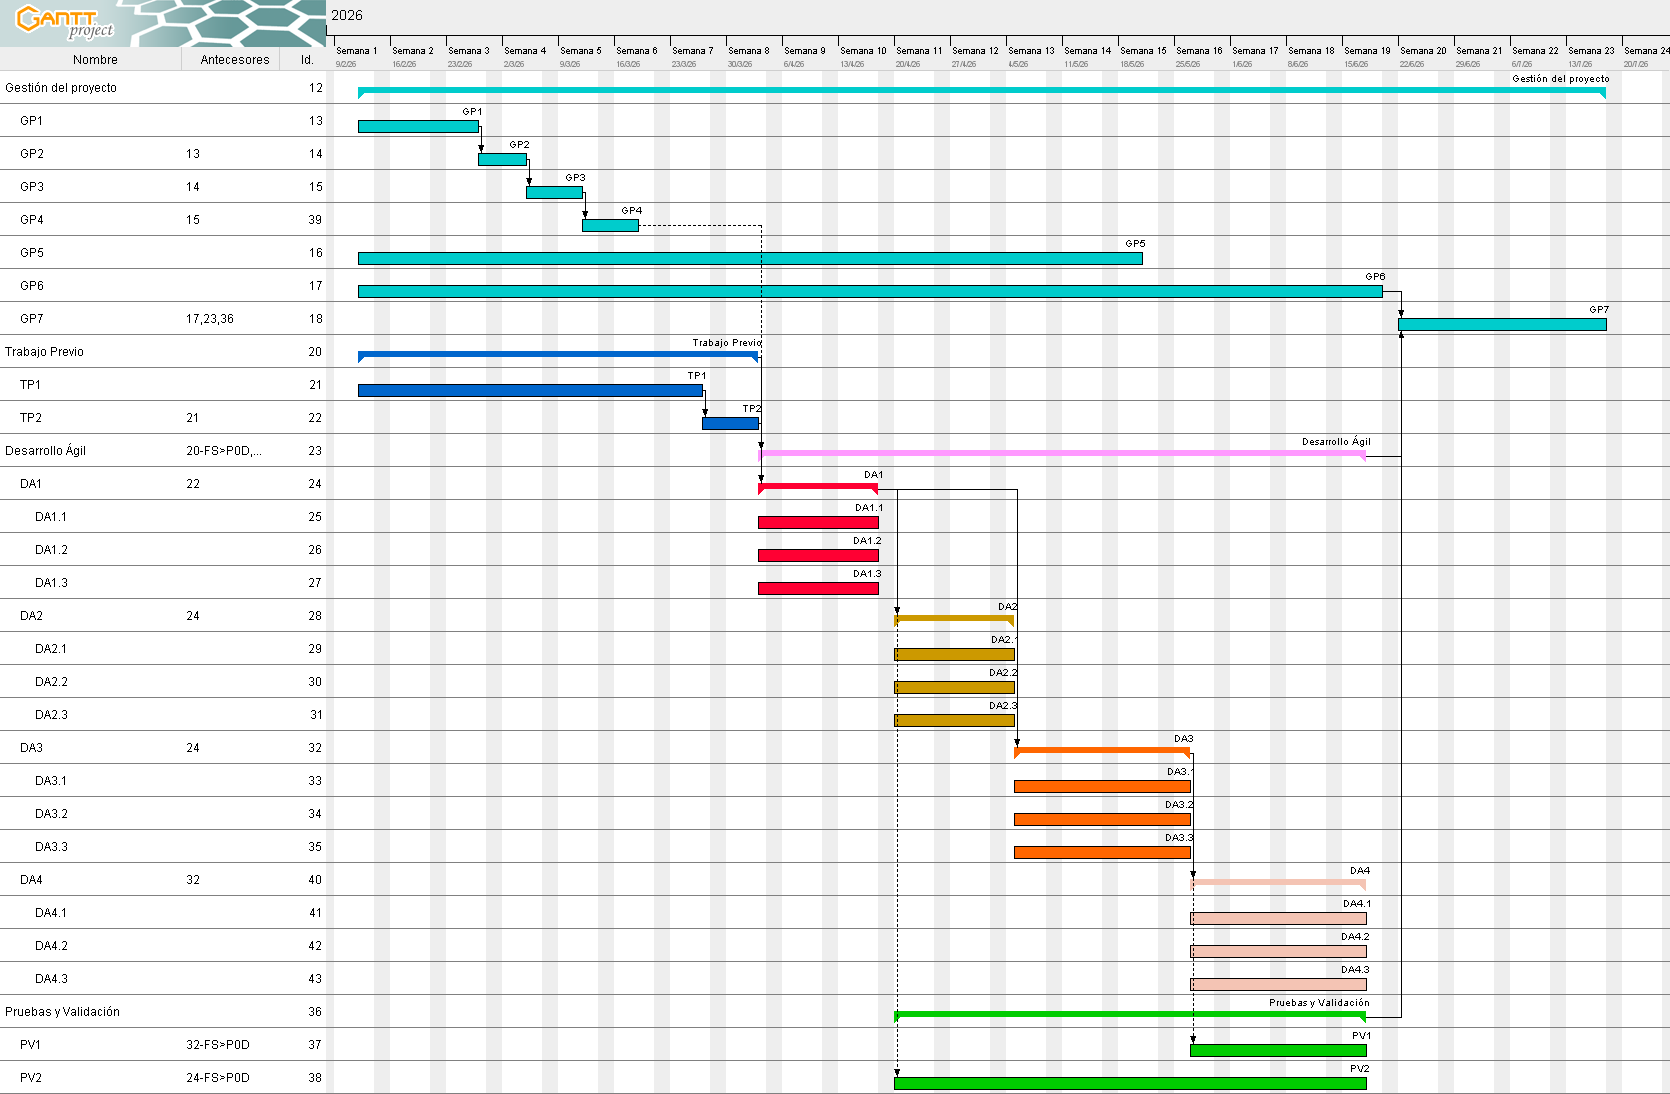
\includegraphics[width=1.5\textwidth]{Gant_Lliurament2.png}
     \caption{Diagrama de Gantt, creado con el software \textit{GanttProject}. Generación propia} 
     \label{fig:heatmap}
    \end{figure}
\end{landscape}

\section{Gestión de riesgos: Planes alternativos y obstáculos}
Durante la planificación y ejecución de este proyecto, se han identificado diversos obstáculos potenciales inherentes al desarrollo con IA. A continuación, se detallan estos riesgos junto con sus respectivos planes alternativos, tal y como dictan las buenas prácticas de gestión ágil de proyectos.

\begin{itemize}
    \item \textbf{Riesgo 1: Cambios repentinos en los requerimientos por parte de la empresa}
    \begin{itemize}
        \item \textbf{Probabilidad:} Media / Alta
        \item \textbf{Tareas afectadas:} Principalmente las fases de Desarrollo Ágil (\textbf{DA1--DA4}), ya que un cambio de requerimientos puede invalidar trabajo ya implementado en cualquier \textit{Sprint}. También se ve afectada la tarea \textbf{GP5} (Reuniones de Seguimiento), que deberá absorber sesiones extraordinarias de re-planificación, y potencialmente \textbf{PV} si los cambios implican redefinir los criterios de validación.
        \item \textbf{Tareas alternativas (Plan B):} Re-evaluación del \textit{Sprint Backlog} actual, congelación del código afectado y re-planificación de los objetivos en una reunión extraordinaria para el siguiente \textit{Sprint}.
        \item \textbf{Afectación a la duración total:} Retraso estimado de 15 horas sobre la planificación original, absorbible en la fase de pruebas (PV).
        \item \textbf{Recursos adicionales necesarios:} Horas extra del autor y disponibilidad del Director del proyecto para una sesión de rediseño.
    \end{itemize}
    
    \vspace{0.3cm}

    \item \textbf{Riesgo 2: Bloqueo tecnológico (Vendor Lock-in) por cambio de precios o políticas en las APIs de los LLMs}
    \begin{itemize}
        \item \textbf{Probabilidad:} Media
        \item \textbf{Tareas afectadas:} El impacto recae principalmente sobre \textbf{DA3} (Habilidades e Integración MCP), donde se construyen los módulos de conexión con las APIs, y sobre \textbf{DA4} (Recuperación de Información y Refinamiento), que depende de integraciones avanzadas con proveedores externos. En menor medida, también puede afectar a \textbf{DA1} si el agente base necesita ser reconectado a un proveedor distinto.
        \item \textbf{Tareas alternativas (Plan B):} Migración del motor cognitivo del sistema hacia modelos \textit{Open Source} (ej. LLaMA o Mistral) ejecutados en local o a través de proveedores alternativos, modificando el módulo de conexión (\textit{wrapper}).
        \item \textbf{Afectación a la duración total:} Aumento de 20 horas en la fase de Integración MCP (DA3).
        \item \textbf{Recursos adicionales necesarios:} Tiempo extra de desarrollo y posible necesidad de hardware local con mayor capacidad de procesamiento (GPU) temporal.
    \end{itemize}
    
    \vspace{0.3cm}

\item \textbf{Riesgo 3: Documentación interna insuficiente para la generación autónoma de código estructurado}
    \begin{itemize}
        \item \textbf{Probabilidad:} Media
        \item \textbf{Tareas afectadas:} Afecta directamente a \textbf{DA1} (implementación del agente Developer, cuya capacidad de escritura se reduciría), \textbf{DA2} (las métricas de evaluación perderían parte de su utilidad si el agente no genera código autónomamente) y \textbf{PV2} (el bucle completo \textit{Human in the Loop} requeriría una mayor intervención manual del autor, alterando la naturaleza de la validación).
        \item \textbf{Tareas alternativas (Plan B):} Reducción del alcance del sistema (\textit{scope downgrade}). Se limitarán las capacidades de escritura del agente \textit{Developer}. El desarrollador humano (usuario) asumirá la implementación directa del código base, mientras que los agentes (\textit{Architect} y \textit{Reviewer}) se reorientarán exclusivamente a tareas de lectura: documentar, auditar la estructura y comprobar la calidad del código manual contra la especificación original.
        \item \textbf{Afectación a la duración total:} Impacto temporal neutro. Las horas ahorradas en el desarrollo de \textit{skills} complejas de escritura para los agentes se reinvertirán en la codificación manual por parte del autor durante el bucle de pruebas (PV).
        \item \textbf{Recursos adicionales necesarios:} Mayor carga de programación manual y esfuerzo cognitivo por parte del autor, al delegar menos carga de implementación en la inteligencia artificial.
    \end{itemize}

    \vspace{0.3cm}

    \item \textbf{Riesgo 4: Limitaciones de control sobre el flujo de orquestación en el ecosistema IDE}
    \begin{itemize}
        \item \textbf{Probabilidad:} Media
        \item \textbf{Tareas afectadas:} Afecta directamente a \textbf{DA1} (implementación del MVP sobre el entorno IDE) y a \textbf{DA3} (Habilidades e Integración MCP), donde se construyen los módulos de orquestación entre agentes. Si las restricciones del IDE resultan insalvables, estas tareas deberán ser rediseñadas.
        \item \textbf{Tareas alternativas (Plan B):} Rediseño de los \textit{prompts} de cada agente para que sean más breves, concisos y con un alcance muy acotado, reduciendo así la tendencia del modelo a desviarse del comportamiento esperado. En este escenario, la coordinación entre agentes recae explícitamente sobre el desarrollador humano, que actúa como orquestador manual del flujo. El inconveniente de esta solución es que exige que el usuario conozca con precisión el proceso de trabajo del sistema para dirigir correctamente a cada agente, lo que aumenta la curva de aprendizaje de la herramienta.
        \item \textbf{Afectación a la duración total:} Aumento estimado de 20 horas en \textbf{DA3} para rediseñar y ajustar los \textit{prompts} de los agentes afectados y documentar el flujo de coordinación manual para el usuario.
        \item \textbf{Recursos adicionales necesarios:} Tiempo de diseño de \textit{prompts} por parte del autor y elaboración de documentación del flujo de uso dirigida al desarrollador.
    \end{itemize}

    \vspace{0.3cm}

    \item \textbf{Riesgo 5: Desbordamiento de la ventana de contexto en proyectos grandes}
    \begin{itemize}
        \item \textbf{Probabilidad:} Media / Alta
        \item \textbf{Tareas afectadas:} Impacta principalmente en \textbf{DA4} (Recuperación de Información y Refinamiento), cuyo objetivo específico es abordar este problema mediante técnicas de \textit{Information Retrieval}. Si se manifiesta antes, también puede bloquear el avance de \textbf{DA1} y \textbf{DA3}, al impedir que los agentes mantengan suficiente contexto para operar correctamente.
        \item \textbf{Tareas alternativas (Plan B):} Aplicar dos estrategias complementarias de reducción de contexto. La primera consiste en implementar resúmenes automáticos o manuales de la conversación, descartando el historial detallado y reteniendo únicamente las decisiones clave ya tomadas. La segunda estrategia consiste en aislar al máximo el alcance de cada agente: en lugar de proporcionar contexto global del proyecto, cada agente opera exclusivamente sobre la \textit{feature} o módulo que tiene asignado, desconociendo intencionadamente el resto de la implementación. Esto mantiene la ventana de contexto acotada y manejable incluso en proyectos grandes.
        \item \textbf{Afectación a la duración total:} Impacto absorbible dentro de las 80 horas ya asignadas a \textbf{DA4}, aunque podría suponer un retraso de hasta 15 horas adicionales si la solución de aislamiento requiere rediseñar la estructura de memoria del sistema.
        \item \textbf{Recursos adicionales necesarios:} Ninguno adicional si se resuelve dentro de \textbf{DA4}; posibles horas extra del autor si la estrategia de aislamiento debe adelantarse a \textit{Sprints} anteriores.
    \end{itemize}

    \vspace{0.3cm}

    \item \textbf{Riesgo 6: Exceso de fricción en el bucle de desarrollo por auditorías demasiado estrictas}
    \begin{itemize}
        \item \textbf{Probabilidad:} Media
        \item \textbf{Tareas afectadas:} Afecta a \textbf{DA3} (implementación del agente Reviewer y sus políticas de auditoría) y a \textbf{PV2} (pruebas del bucle completo \textit{Human in the Loop}), donde se evalúa empíricamente si el sistema resulta usable o frustrante para el desarrollador.
        \item \textbf{Tareas alternativas (Plan B):} Rediseño del agente \textit{Reviewer} para implementar niveles de severidad en las auditorías (errores críticos bloqueantes vs. advertencias no bloqueantes), permitiendo al usuario continuar el desarrollo ante desviaciones menores y reservando los bloqueos para incumplimientos graves de la especificación.
        \item \textbf{Afectación a la duración total:} Aumento de aproximadamente 10 horas en \textbf{DA3} para recalibrar y probar los umbrales de tolerancia del agente \textit{Reviewer}.
        \item \textbf{Recursos adicionales necesarios:} Sesiones de prueba adicionales con el autor actuando como usuario final para validar que el nuevo umbral resulta equilibrado.
    \end{itemize}
\end{itemize}

\newpage

\section{Gestión económica}
En este apartado plantearemos los distintos costes que se prevé que aparecerán a lo largo del desarrollo del proyecto.

\subsection{Coste del personal}
Aplicando el \textit{feedback} de la anterior entrega de GEP, vamos a dividir este apartado en distintos roles. Cada uno tendrá un coste por hora determinado, y visitando el diagrama de Gantt y las tablas con las horas asignadas a cada tarea y sus recursos personales adjuntados, calcularemos el total de cada uno de estos roles. Adicionalmente, se mostrarán tanto los salarios netos como los brutos - añadida la contribución de 30\verb|%| a la Seguridad Social (SS) -, y cuando se haga la suma total de los costes, se utilizará obviamente el salario bruto.

\begin{table}[H]
    \centering
    \begin{tabularx}{\textwidth}{|X|c|c|}
         \hline
         \textbf{Rol} & \textbf{Salario Neto} & \textbf{Salario Bruto (+ SS)}\\ 
         \hline
         \hline
         Jefe del Proyecto (Programador senior) & 20,15€/h & 26,20€/h \\
         Investigador y documentador & 16,04€/h & 20,85€/h \\
         Programador junior &  11,48€/h & 14,92€/h \\
         Testers & 14,72€/h & 19,17€/h \\
         \hline
    \end{tabularx}
    \caption{Costes de personal por hora según el rol asumido. Generación propia. Basada en información extraída de \cite{indeed_salarios}}.
    \label{tab:costes_personal}
\end{table}

\subsection{Coste por actividad}
Repasaremos las actividades presentadas en el entregable anterior, estudiaremos los recursos humanos invertidos en dicha actividad, y calcularemos el coste de cada una.
\subsubsection{Gestión del proyecto}
Esta se ha estimado que durará unas 167 horas en total. Dando por hecho que se desarrolla en un 25\verb|%| por el \textit{Jefe del Proyecto} y el restante 75\verb|%| por el \textit{Investigador/Documentador}, el coste humano de esta tarea es de: 
\begin{equation}
\centering
Coste GP = (0{.}25*26{.}2 \verb|€|/h + 0{.}75*20{.}85 \verb|€|/h)*167h = 3705{.}32\verb|€|
\end{equation}
\subsubsection{Trabajo Previo}
Esta actividad se estima que es de unas 50 horas. Requiere un estudio del estado del arte, y planificación del flujo del funcionamiento del proyecto. Las 30 horas de investigación del estudio del arte podrían estar desarolladas por el \textit{Investigador/Desarrollador}, mientras que la planificación del proyecto se llevaría a cabo por el \textit{Jefe del Proyecto}, por lo que 20 horas de su parte.
\begin{equation}
    Coste TP = 20h * 26{.}2\verb|€/h| + 30h * 20{.}85\verb|€|/h = 1149{.}5\verb|€|
\end{equation}
\subsubsection{Desarrollo Ágil}
Como se hizo en la entrega anterior, el desarrollo ágil (DA) se dividirá en DA1, DA2, DA3 y DA4. Basándonos en la naturaleza de cada iteración, repartiremos la carga de trabajo entre los distintos roles definidos para estimar su coste:

\begin{itemize}
    \item \textbf{DA1 (Sprint 1 - MVP):} Consta de 50 horas en total. Al tratarse de la implementación técnica de los agentes base en el entorno IDE, asignaremos la totalidad de estas horas al \textit{Programador junior}.
    \begin{equation*}
        Coste DA1 = 50h * 14{.}92\verb|€|/h = 746\verb|€|
    \end{equation*}
    
    \item \textbf{DA2 (Sprint 2 - Métricas de Evaluación):} Consta de 50 horas. Las 15 horas iniciales de investigación y selección de métricas serán llevadas a cabo por el \textit{Investigador y documentador}, mientras que las 35 horas restantes de desarrollo de scripts e integración recaerán sobre el \textit{Programador junior}.
    \begin{equation*}
        Coste DA2 = 15h * 20{.}85\verb|€|/h + 35h * 14{.}92\verb|€|/h = 836\verb|€|
    \end{equation*}
    
    \item \textbf{DA3 (Sprint 3 - Habilidades e Integración MCP):} De las 80 horas estimadas, 65 horas se dedicarán al desarrollo de \textit{Agent Skills} y protocolos MCP por parte del \textit{Programador junior}. Las 15 horas restantes, dedicadas al análisis de errores complejos y mejoras de estabilidad, requerirán la experiencia y supervisión del \textit{Jefe del Proyecto}.
    \begin{equation*}
        Coste DA3 = 65h * 14{.}92\verb|€|/h + 15h * 26{.}2\verb|€|/h = 1362{.}8\verb|€|
    \end{equation*}
    
    \item \textbf{DA4 (Sprint 4 - Recuperación de Información y Refinamiento):} Cuenta con 80 horas totales. Asignaremos 20 horas al \textit{Investigador y documentador} para analizar y diseñar las técnicas de \textit{Information Retrieval}, y las 60 horas restantes al \textit{Programador junior} para la integración final y resolución de \textit{bugs}.
    \begin{equation*}
        Coste DA4 = 20h * 20{.}85\verb|€|/h + 60h * 14{.}92\verb|€|/h = 1312{.}2\verb|€|
    \end{equation*}
\end{itemize}

Sumando los costes de los cuatro \textit{Sprints}, obtenemos el coste total de los recursos humanos para la fase de Desarrollo Ágil:
\begin{equation}
    Coste DA = 746\verb|€| + 836\verb|€| + 1362{.}8\verb|€| + 1312{.}2\verb|€| = 4257\verb|€|
\end{equation}
\subsubsection{Pruebas y Validación}
Se estimó que en total esta tarea tomaría unas 60 horas a lo largo del proyecto. De estas 60 horas, todas ellas serian asignadas al Tester.

\begin{equation}
    Coste PV = 60h * 19{.}17\verb|€|/h = 1150{.}2\verb|€|
\end{equation}
\subsection{Costes genéricos}
En este apartado se referenciarán los costes que no se pueden asignar a una actividad específica, sino que están presentes a lo largo de todo el desarrollo. Estos incluyen los gastos de infraestructura, licencias de software y la amortización del equipo físico utilizado.

\subsubsection{Costes estructurales}
Los costes estructurales contemplan los gastos derivados del uso de un espacio de trabajo físico, así como los suministros básicos necesarios para llevar a cabo el desarrollo. Asumiendo que el proyecto tiene una duración estimada de 4,5 meses (desde mediados de febrero hasta principios de julio), se han estimado los siguientes gastos mensuales:

\begin{itemize}
    \item \textbf{Alquiler de la oficina:} Se asume el alquiler de un puesto en un espacio de \textit{coworking} o la parte proporcional de una oficina compartida, estimado en 150\verb|€|/mes. \cite{barcelona_coworking}
    \item \textbf{Electricidad:} Consumo derivado de los equipos informáticos, iluminación y climatización del espacio de trabajo, estimado en 50\verb|€|/mes. \cite{naturgy_precios}
    \item \textbf{Suministros adicionales:} Gastos de conectividad a Internet de alta velocidad y agua, calculados en 40\verb|€|/mes.
\end{itemize}

En total, el coste estructural mensual asciende a 240\verb|€|. Por lo tanto, el cálculo para los 4,5 meses de duración del proyecto es el siguiente:

\begin{equation}
    Coste Estructural = 4{.}5 \text{ meses} * 240\verb|€|/\text{mes} = 1080\verb|€|
\end{equation}

\subsubsection{Costes de \textit{Software}}
El ecosistema tecnológico del proyecto se apoya en diversas herramientas. Afortunadamente, muchas de ellas cuentan con licencias gratuitas o versiones académicas sin coste (como Git, GitHub, VSCode, Odoo y Microsoft Teams). Sin embargo, el núcleo de este TFG requiere el uso de inteligencia artificial, lo que implica costes de suscripción y consumo de APIs (Claude Code, GitHub Copilot y servicios de Microsoft Azure / OpenAI).

Se ha estimado un presupuesto de consumo mensual para estas herramientas:
\begin{itemize}
    \item \textbf{GitHub Copilot:} 10\verb|€|/mes. \cite{github_pricing}
    \item \textbf{Claude:} 20\verb|€|/mes. \cite{claude_plans}
    \item \textbf{Consumo de APIs LLM (Azure/OpenAI/Anthropic):} 30\verb|€|/mes.
\end{itemize}
\begin{equation}
    Coste Software = (10\verb|€|/\text{mes}+ 20\verb|€|/\text{mes} + 30\verb|€|/\text{mes}) * 4{.}5 \text{ meses} = 270\verb|€|
\end{equation}

\subsubsection{Costes de \textit{Hardware}}
Para calcular el coste del hardware, no se debe imputar el precio total de compra de los equipos, ya que estos no agotarán su vida útil exclusivamente con este proyecto. Se debe calcular su amortización. 

La fórmula de amortización se define dividiendo el precio del equipo entre sus horas de vida útil, y multiplicando el resultado por las horas dedicadas al TFG (estimadas en 540 horas en total). Se asume una vida útil de 4 años para los equipos informáticos (aproximadamente 220 días laborables al año, a 8 horas diarias = 7040 horas).

\begin{table}[H]
    \centering
    \begin{tabularx}{\textwidth}{|X|c|c|c|}
         \hline
         \textbf{Dispositivo} & \textbf{Precio Compra} & \textbf{Vida Útil (h)} & \textbf{Amortización (540h)} \\ 
         \hline
         \hline
         Estación de trabajo (PC) & 1500€ & 7040h & 115,06€ \\
         Monitor externo & 200€ & 7040h & 15,34€ \\
         Periféricos (Teclado, ratón, audio) & 100€ & 7040h & 7,67€ \\
         \hline
         \textbf{Total} & \textbf{1800€} & - & \textbf{138,07€} \\
         \hline
    \end{tabularx}
    \caption{Cálculo de la amortización de los recursos de \textit{Hardware}. Generación propia.}
    \label{tab:amortizacion_hardware}
\end{table}

\begin{equation}
    Coste Hardware = 115{.}06\verb|€| + 15{.}34\verb|€| + 7{.}67\verb|€| = 138{.}07\verb|€|
\end{equation}

Sumando todos los componentes detallados en esta subsección, el total de costes genéricos asciende a:
\begin{equation}
    Total Genericos = 1080\verb|€| + 270\verb|€| + 138{.}07\verb|€| = 1488{.}07\verb|€|
\end{equation}

\subsection{Contingencias e imprevistos}
En el desarrollo de cualquier proyecto de ingeniería informática, es fundamental disponer de un margen económico para hacer frente a posibles desviaciones temporales o problemas técnicos. Este margen se divide en dos partidas: las contingencias (para riesgos desconocidos) y los imprevistos (para riesgos ya identificados).

\subsubsection{Contingencias}
La partida de contingencias actúa como un fondo de reserva general. Dado que el proyecto se basa en la integración de Inteligencia Artificial (LLMs) y herramientas en constante evolución, existe un grado de incertidumbre inherente. Aplicando las buenas prácticas de gestión de proyectos informáticos, se establece un margen de contingencia del 15\verb|%| sobre la suma total de los costes de personal y los costes genéricos estimados hasta el momento.
\begin{equation}
    Coste Contingencias = (Coste Personal + Coste Genericos) * 0{.}15
\end{equation}

\subsubsection{Imprevistos}
Por otro lado, la partida de imprevistos cuantifica económicamente los riesgos específicos que ya fueron identificados y analizados en el Entregable 2. El coste que se añade al presupuesto se calcula multiplicando el coste del plan de acción alternativo (Plan B) por la probabilidad estimada de que el riesgo ocurra.

\begin{itemize}
    \item \textbf{Riesgo 1: Cambios repentinos en los requerimientos.} La probabilidad de ocurrencia se estimó como Media/Alta (asignaremos un 60\verb|%|). El plan de mitigación contempla un retraso de 15 horas, implicando re-planificación y desarrollo. Asignaremos 5 horas al \textit{Jefe de Proyecto} (26,20\verb|€|/h) y 10 horas al \textit{Programador junior} (14,92\verb|€|/h).
    \begin{equation*}
        Coste R1 = ((5h * 26{.}20\verb|€|/h) + (10h * 14{.}92\verb|€|/h)) * 0{.}60 = 280{.}2\verb|€| * 0{.}60 = 168{.}12\verb|€|
    \end{equation*}
    \textbf{Impacto: Medio}
    
    \item \textbf{Riesgo 2: Bloqueo tecnológico (Vendor Lock-in) en APIs LLM.} La probabilidad es Media (50\verb|%|). El plan alternativo es la migración a modelos \textit{Open Source}, con un impacto de 20 horas de desarrollo (\textit{Programador junior}) y el alquiler puntual de hardware en la nube con GPU (estimado en 100\verb|€|).
    \begin{equation*}
        Coste R2 = ((20h * 14{.}92\verb|€|/h) + 100\verb|€|) * 0{.}50 = 398{.}4\verb|€| * 0{.}50 = 199{.}2\verb|€|
    \end{equation*}
    \textbf{Impacto: Medio}

    \item \textbf{Riesgo 3: Documentación interna insuficiente.} Probabilidad Media (50\verb|%|). El plan alternativo consiste en realizar un \textit{scope downgrade} (reducir capacidades de escritura de los agentes). Al tener un impacto temporal neutro (las horas no invertidas en IA se invierten en programación manual), no genera un coste económico extra en el presupuesto.
    \begin{equation*}
        Coste R3 = 0\verb|€| * 0{.}50 = 0\verb|€|
    \end{equation*}
    \textbf{Impacto: Bajo}
\end{itemize}

Sumando los valores obtenidos, calculamos el fondo total reservado para imprevistos:
\begin{equation}
    Total Imprevistos = 168{.}12\verb|€| + 199{.}2\verb|€| + 0\verb|€| = 367{.}32\verb|€|
\end{equation}

\subsection{Coste total}
Una vez estimados todos los gastos asociados al desarrollo del proyecto, tanto directos (personal) como indirectos (genéricos), y habiendo reservado los fondos necesarios para contingencias e imprevistos, podemos definir el presupuesto final. 

A continuación, se presenta una tabla resumen con la consolidación de todas las partidas económicas calculadas previamente:

\begin{table}[H]
    \centering
    \begin{tabular}{|l|c|}
         \hline
         \textbf{Concepto} & \textbf{Coste Estimado} \\ 
         \hline
         \hline
         Coste de Personal (GP, TP, DA, PV) & 10.262,02€ \\
         Costes Genéricos (Estructurales, Software, Hardware) & 1.488,07€ \\
         \hline
         \textbf{Subtotal (Base del proyecto)} & \textbf{11.750,09€} \\
         \hline
         Contingencias (15\verb|%| sobre el Subtotal) & 1.762,52€ \\
         Imprevistos (Riesgos evaluados) & 367,32€ \\
         \hline
         \hline
         \textbf{PRESUPUESTO TOTAL} & \textbf{13.879,93€} \\
         \hline
    \end{tabular}
    \caption{Presupuesto total estimado del proyecto. Generación propia.}
    \label{tab:coste_total}
\end{table}

\subsection{Control de gestión}
Para asegurar la viabilidad económica del Trabajo de Fin de Grado y evitar que el proyecto supere el presupuesto establecido, es estrictamente necesario aplicar un control de gestión continuo. Al utilizar una metodología ágil (SCRUM), este control se realizará al finalizar cada iteración o \textit{Sprint}, así como en las reuniones de seguimiento estipuladas.

El control se basará en comparar los valores estimados en este documento con los gastos y horas reales consumidas. Para cada indicador se define su fórmula de cálculo y los criterios de actuación concretos en función de la magnitud de la desviación detectada:

\begin{itemize}
    \item \textbf{Desviación de horas por tarea:} Mide si se ha invertido más o menos tiempo del planificado en una tarea concreta.
    \begin{equation}
        Desviaci\acute{o}n\ Horas = Horas\ Estimadas - Horas\ Reales
    \end{equation}
    \textbf{Criterio de actuación:}
    \begin{itemize}
        \item Desviación entre 0 y $-$10\%: dentro del margen tolerable. Se registra como nota en la revisión del \textit{Sprint} pero no requiere acción inmediata.
        \item Desviación entre $-$10\% y $-$20\%: se analiza la causa en la reunión de seguimiento con el director y se ajusta la estimación de las tareas pendientes del mismo bloque.
        \item Desviación superior al $-$20\%: se convoca una sesión extraordinaria de re-planificación, se re-prioriza el \textit{Sprint Backlog} y se eliminan o posponen las subtareas de menor valor del incremento actual.
    \end{itemize}

    \item \textbf{Desviación de coste de personal:} Calcula el impacto económico de la desviación de horas, multiplicándolo por el salario bruto del rol implicado.
    \begin{equation}
        Desviaci\acute{o}n\ Coste\ Personal = (Horas\ Estimadas - Horas\ Reales) * Coste\ Rol
    \end{equation}
    \textbf{Criterio de actuación:}
    \begin{itemize}
        \item Desviación acumulada inferior a $-$300\verb|€|: absorbible con el fondo de contingencias (15\%), sin acción adicional.
        \item Desviación acumulada entre $-$300\verb|€| y $-$800\verb|€|: se activa el fondo de contingencias y se restringe el alcance de las tareas de menor prioridad del bloque en curso.
        \item Desviación acumulada superior a $-$800\verb|€|: se aplica un \textit{scope downgrade} formal, eliminando funcionalidades secundarias para reconducir el presupuesto hacia los objetivos críticos del proyecto.
    \end{itemize}

    \item \textbf{Desviación de costes genéricos:} Controla si herramientas de software, hardware o infraestructura han sufrido variaciones de precio (por ejemplo, subida de tarifas en las APIs de los LLMs).
    \begin{equation}
        Desviaci\acute{o}n\ Gen\acute{e}ricos = Coste\ Gen\acute{e}rico\ Estimado - Coste\ Gen\acute{e}rico\ Real
    \end{equation}
    \textbf{Criterio de actuación:}
    \begin{itemize}
        \item Desviación puntual inferior a $-$30\verb|€|/mes: se registra y monitoriza. Si persiste más de dos meses consecutivos, se revisan alternativas.
        \item Desviación sostenida o superior a $-$30\verb|€|/mes: se evalúa la sustitución de la herramienta afectada por una alternativa gratuita u \textit{open source} equivalente (por ejemplo, migrar a un proveedor de LLM alternativo en caso de subida de tarifas de APIs).
    \end{itemize}

    \item \textbf{Consumo del fondo de imprevistos:} Evalúa cuánto remanente queda del fondo de emergencias calculado. Si el resultado es negativo, significa que se ha agotado el presupuesto de seguridad.
    \begin{equation}
        Estado\ Imprevistos = Total\ Imprevistos\ Estimado - Coste\ Imprevistos\ Consumido
    \end{equation}
    \textbf{Criterio de actuación:}
    \begin{itemize}
        \item Remanente superior al 50\% (más de 183\verb|€| disponibles): situación bajo control, sin cambios en el plan.
        \item Remanente entre el 0\% y el 50\%: se congela el uso del fondo para nuevos imprevistos menores y se activa el fondo de contingencias para cubrir desviaciones adicionales.
        \item Remanente negativo (fondo agotado): se aplica de inmediato un \textit{scope downgrade} de las funcionalidades con mayor riesgo económico y se notifica al director del proyecto para valorar conjuntamente medidas extraordinarias.
    \end{itemize}
\end{itemize}

\newpage

\section{Informe de sostenibilidad}

\subsection{Autoevaluación de la competencia}
Tras realizar la encuesta de autoevaluación, identifico un perfil técnico sólido pero con carencias formativas en la gestión de la sostenibilidad. Uno de mis puntos fuertes es el compromiso con la eficiencia técnica y el orden del código (\textit{Green Computing}), lo que garantiza soluciones robustas y mantenibles a largo plazo. No obstante, el cuestionario ha evidenciado que durante la carrera me han faltado asignaturas que profundicen en métricas de sostenibilidad medioambiental, económica y social.

Esta falta de base académica ha sido mi principal punto débil al afrontar la estimación de costes y riesgos de este proyecto. Sin embargo, mediante un proceso de aprendizaje autónomo durante la planificación, he comprendido la importancia crítica de estos conceptos para gestionar adecuadamente un proyecto de cierto calibre como puede ser un TFG. Esta reflexión me ha permitido adoptar una visión más empática de la ingeniería, utilizando la metodología SDD no solo para buscar la eficiencia, sino para prevenir el \textit{burnout} y fomentar la sostenibilidad social del equipo.

\subsection{Dimensión económica}
% Añadir beneficios del proyecto. ¿Porque puede merecer la pena gastarse 14.000€ en esto?
\textbf{PPP:} El coste total del proyecto se estima en 13.879,93€. Tras reflexionar sobre este presupuesto, considero que es realista y competitivo para un desarrollo de 540 horas que integra tecnologías punteras de IA. La optimización del gasto se logra mediante el uso de herramientas de código abierto y un modelo de pago por uso para las APIs, centrando la inversión en el valor del esfuerzo humano y la investigación.

\textbf{Vida Útil:} Actualmente, la industria aborda el desarrollo asistido por IA de forma impulsiva (Code-Driven), lo que reduce costes iniciales pero dispara los de mantenimiento debido a la deuda técnica. Esta solución basada en SDD mejora económicamente este escenario al reducir dicha deuda desde la fase de planificación. Idealmente, el ahorro en tiempo de comprensión y corrección de errores debería amortizar la inversión inicial del proyecto.

\textbf{Mantenimiento:} El coste operativo tras la entrega es mínimo, estimado en aproximadamente 120€/mes. Este importe cubre los costes de suscripciones a las APIs de IA (GitHub, Anthropic, ...) y unas 4 horas mensuales de soporte técnico de un \textit{programador junior} para actualizaciones menores y ajustes varios.
\begin{equation}
    CosteMantenimiento = 60\verb|€|/mes + 4h/mes * 14{.}92\verb|€|/h = 119{.}68\verb|€|
\end{equation}

\subsection{Dimensión social}
\textbf{PPP:} A nivel personal, este proyecto es un catalizador en mi formación. Me permite consolidar conocimientos técnicos en la orquestación de LLMs y, simultáneamente, adquirir habilidades críticas en gestión económica y metodologías ágiles (SCRUM), competencias que han demostrado ser tan vitales como la propia programación.

\textbf{Vida Útil:} Existe una necesidad real en el mercado debido al creciente estrés y frustración profesional que genera trabajar con bases de código incoherentes. La metodología SDD mejora la calidad de vida de los programadores al obligar a establecer especificaciones claras, reduciendo el caos y fomentando un entorno laboral más estructurado y colaborativo.

\subsection{Dimensión ambiental}
\textbf{PPP:} El impacto ambiental proviene del consumo eléctrico de los equipos durante las 540 horas de trabajo y el uso de servidores en la nube para las APIs. Para minimizar este impacto, se ha optado por reutilizar hardware personal y planificar un desarrollo local mediante WSL que limite las peticiones innecesarias a la red durante las fases iniciales de pruebas.

\textbf{Vida Útil:} Este sistema actúa como un optimizador de recursos. Mientras que las soluciones actuales fomentan un bucle de \verb|"|ensayo y error\verb|"| que multiplica las peticiones a los LLMs, el enfoque SDD permite ir \verb|"|al grano\verb|"| con código estructurado. Esto se traduce en una reducción drástica de llamadas a los modelos masivos a largo plazo, disminuyendo el consumo energético global de los centros de datos.


% HOLA DAVID, HE ELIMINADO EL APARTADO DE REFERENCIAS porque según los documentos de ejemplo porpocionados por mi universidad, en esta entrega que solo es documentación no eran necesarias!

%\addcontentsline{toc}{section}{Referencias}

%\bibliographystyle{plain} 

%\bibliography{references1}

\newpage
\addcontentsline{toc}{section}{Referencias}

\begin{thebibliography}{99}

    \bibitem{ostroff_agile_2004}
    Ostroff, J., Makalsky, D., y Paige, R. (2004). \textit{Agile Specification-Driven Development}.
    En: \textit{Extreme Programming and Agile Methods}. Springer.
    \url{https://doi.org/10.1007/978-3-540-24853-8_12}

    \bibitem{github_spec_kit}
    GitHub. (2025). \textit{github/spec-kit Repository}.
    Recuperado de: \url{https://github.com/github/spec-kit}. Accedido el 24/02/2026

    \bibitem{jama_requirements}
    Jama Software. (2026). \textit{What is Requirements Gathering in Software Engineering?}
    Recuperado de: \url{https://www.jamasoftware.com/requirements-management-guide/requirements-gathering-and-management-processes/what-is-requirements-gathering/}. Accedido el 25/02/2026

    \bibitem{vscode_agents}
    Microsoft. (2026). \textit{Using agents in Visual Studio Code}.
    Recuperado de: \url{https://code.visualstudio.com/docs/copilot/agents/overview}. Accedido el 25/02/2026

    \bibitem{agentskills_home}
    AgentSkills. (2026). \textit{AgentSkills Documentation}.
    Recuperado de: \url{https://agentskills.io/home}. Accedido el 25/02/2026

    \bibitem{buildermethods_agent_os}
    Builder Methods. (2025). \textit{buildermethods/agent-os}.
    Recuperado de: \url{https://github.com/buildermethods/agent-os}. Accedido el 25/02/2026

    \bibitem{github_copilot_docs}
    GitHub. (2026). \textit{GitHub Copilot documentation}.
    Recuperado de: \url{https://docs.github.com/en/copilot}. Accedido el 25/02/2026

    \bibitem{cursor_ai}
    Cursor. (2026). \textit{Cursor: The best way to code with AI}.
    Recuperado de: \url{https://cursor.com}. Accedido el 25/02/2026

    \bibitem{modul2_1}
    Departament d'Organització d'Empreses (FIB). \textit{Mòdul 2.1.b -- Gestión ágil de proyectos}.
    Universitat Politècnica de Catalunya.

    \bibitem{indeed_salarios}
    Indeed. (2026). \textit{Guía de salarios en España: Explorar sueldos por cargo y ubicación}.
    Recuperado de: \url{https://es.indeed.com/career/salaries}. Accedido el 08/03/2026

    \bibitem{barcelona_coworking}
    Barcelona Life. (2026). \textit{Guide to Coworking Spaces in Barcelona: Shared Offices}.
    Disponible en: \url{https://www.barcelona-life.com/barcelona-coworking-spaces}. Accedido el 10/03/2026

    \bibitem{naturgy_precios}
    Naturgy. (2026). \textit{Precio de la luz y tarifas eléctricas para el hogar}.
    Disponible en: \url{https://www.naturgy.es/hogar/luz/precio_de_la_luz}. Accedido el 10/03/2026

    \bibitem{github_pricing}
    GitHub. (2026). \textit{GitHub Pricing Plans: Personal and Business}.
    Recuperado de: \url{https://github.com/pricing}. Accedido el 09/03/2026

    \bibitem{claude_plans}
    Anthropic. (2026). \textit{Choosing a Claude plan: Free, Pro, and Team}.
    Recuperado de: \url{https://support.claude.com/en/articles/11049762-choosing-a-claude-plan}. Accedido el 09/03/2026

\end{thebibliography}

\end{document}